\documentclass[preprint, 10pt]{elsarticle}

\newcommand{\mcaption}[2]{\caption{\small \em #1}\label{#2}}
\newcommand{\secref}[1]{\ref{#1}}

\usepackage{amsfonts}
\usepackage[fleqn,reqno]{amsmath}
\usepackage{amssymb}
\usepackage[titletoc]{appendix}
\usepackage{enumitem}
\usepackage{filecontents}
\usepackage[top=1.2in,bottom=1.2in,left=1in, right=1in]{geometry}
\usepackage{graphics}
\usepackage{lineno}
%\usepackage{showkeys} %To see the labels for now.  Will remove later
\usepackage{pgfplots}
\usepackage{tikz}
\usepackage{todonotes}

\usetikzlibrary{arrows}


%%%%%%  pdftex  %%%%%%%%%%%%%%%%%%%%%%%%%%%%%%%%%%%%%%%%%%%%%%%%%%%%%%
\usepackage[pagebackref=false,bookmarks=false]{hyperref} 

\hypersetup{
  bookmarksnumbered=true,
  bookmarksopen=false,
  hypertexnames=false,      
  breaklinks=true,          
  unicode=false,
  pdffitwindow=true,        
  pdfnewwindow=true,        
  colorlinks=true,         
  linkcolor=dblue,
  anchorcolor=red,
  citecolor=dorange,
  filecolor=magenta,
  urlcolor=dblue,
  pdfstartview = FitH,
  pdfkeywords = {},
  pdfcreator = {LaTeX with hyperref package}
}

\newcommand{\bd}{{\partial}}
\newcommand{\cc}{{\mathbf{c}}}
\newcommand{\DD}{{\mathcal{D}}}
\newcommand{\eeta}{{\boldsymbol\eta}}
\newcommand{\ff}{{\mathbf{f}}}
\newcommand{\grad}{{\nabla}}
\newcommand{\llambda}{{\boldsymbol\lambda}}
\newcommand{\nn}{{\mathbf{n}}}
\newcommand{\NN}{{\mathcal{N}}}
\newcommand{\pderiv}[2]{\frac{\partial #1}{\partial #2}}
\newcommand{\rr}{{\mathbf{r}}}
\newcommand{\RR}{{\mathbb{R}}}
\renewcommand{\ss}{{\mathbf{s}}}
\newcommand{\ssigma}{{\boldsymbol\sigma}}
\newcommand{\uu}{{\mathbf{u}}}
\newcommand{\UU}{{\mathbf{U}}}
\newcommand{\vv}{{\mathbf{v}}}
\newcommand{\xx}{{\mathbf{x}}}
\newcommand{\xxi}{{\boldsymbol{\xi}}}
\newcommand{\yy}{{\mathbf{y}}}

\begin{document}

\title{Methods paper for rigid bodies}

\author[Lukas]{Lukas Bystircky}
\author[Lukas]{Sachin Shanbhag}
\author[Bryan]{Bryan D.~Quaife}
\address[Lukas]{Department of Scientific Computing, Florida State University,
Tallahassee, FL, 32306.}
\address[Bryan]{Department of Scientific Computing and Geophysical Fluid
Dynamics Institute, Florida State University, Tallahassee, FL, 32306.}

\begin{abstract} 
We consider suspensions of rigid bodies in two dimensions \ldots
\end{abstract}

\begin{keyword}
  Stokes flow \sep Boundary integral method \sep Rigid body suspensions 
\end{keyword}

\maketitle





%%%%%%%%%%%%%%%%%%%%%%%%%%%%%%%%%%%%%%%%%%%%%%%%%%%%%%%%%%%%%%%%%%%%%%%
\section{Introduction\label{s:intro}}

\todo[inline]{Bryan will write this section}

This is a methods paper
\begin{itemize}
  \item Boundary integral equation formulation
  \item STIV
  \item FMM
  \item Near-singular integration
  \item Pressure and energy dissipation calculations
  \item Time integrator
\end{itemize}




%%%%%%%%%%%%%%%%%%%%%%%%%%%%%%%%%%%%%%%%%%%%%%%%%%%%%%%%%%%%%%%%%%%%%%%
\section{Formulation\label{s:formulation}} 



\subsection{Problem Formulation}

We consider a suspension of rigid particles flowing in a two dimensional
domain, $\Omega$ with boundary $\partial\Omega$.  The domain may be bounded or
unbounded, and may be multiply-connected. The enclosures inside $\Omega$ are fixed solid walls or mobile rigid particles. The boundaries of solid walls are denoted $\Gamma_i$, $1\leq i \leq M_w$, the union of these boundaries is denoted $\Gamma$.  The boundaries of rigid particles are denoted $\gamma_j$, $1\leq j\leq M_p$ and their union is denoted $\gamma$. If the geometry is
bounded, the overall enclosing boundary is $\Gamma_0$.  Thus we can express the boundary as,
\begin{equation} \partial\Omega =\Gamma_0\cup \Gamma \cup \gamma,\end{equation}
where $\Gamma_0$ is excluded if the geometry is unbounded. Each solid wall has a center $\cc^\Gamma_i$ and each rigid particle has a center $\cc^\gamma_j$ and an orientation angle $\theta^\gamma_j$.  Finally, each solid wall and rigid
particle will have a net force and torque that they apply to the fluid denoted $\FF^\Gamma_i$ and $L^\Gamma_i$ for walls, and $\FF^\gamma_j$ and $L^\gamma_j$ for particles respectively.  A schematic
of the geometry is in Figure~\ref{fig:geomSchematic}

%
%The fluid will be in a domain $\Omega$ with a boundary
%$\partial\Omega$. The boundary $\partial\Omega$ is the union of the
%surfaces of $N$ suspended particles each with a boundary $\gamma_k$,
%$1\leq k \leq N$, the surfaces of $M$ solid walls each with boundary,
%$\Gamma_\ell$, $1\leq\ell\leq M$ and optionally a containing wall
%denoted $\Gamma_0$. The suspended particles are all rigid and at each
%time step we will solve for their translational velocity
%$\mathbf{u}^{\tau}_k$ and angular velocity $\omega_k$, allowing us to
%update their centers and orientations, $\mathbf{c}_k$ and $\theta_k$
%respectively. Particles and interior walls will be undergoing a net
%force $\mathbf{F}_{k/\ell}$  and torque $L_{k/\ell}$. 

\begin{figure}[!h]
\begin{center}
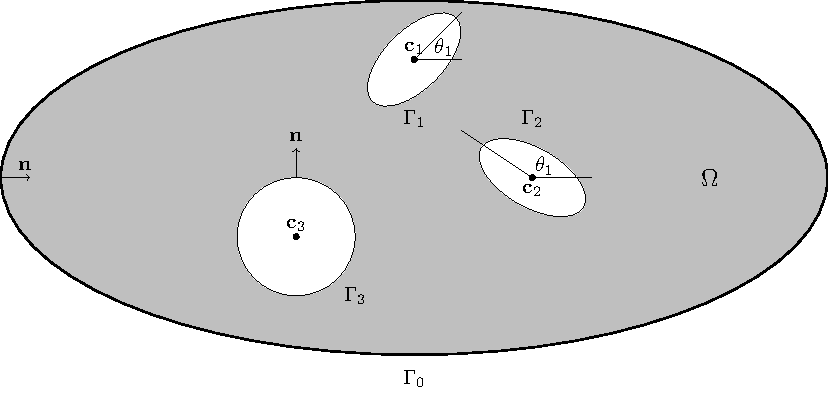
\includegraphics{figures/multiply_connected.pdf}
\end{center}
\caption{\label{fig:geomSchematic}Sketch of a possible domain $\Omega$.
  $\gamma_1$ and $\gamma_2$ enclose particles, while $\Gamma_1$ is a
  solid wall. The outer boundary $\Gamma_0$ need not be present.  The
  vector $\mathbf{n}$ is the unit normal vector pointing into the fluid
  domain.}
\end{figure}

%%%%%%%%%%%%%%%%%%%%%%%%%%%%%%%%%%%%%%%%%%%%%%%%%%%%%%%%%%%%%%%%%%%%%%%%%%%%%%%
\subsection{Governing Equations}\label{sec:governing}
At the continuum level the motion of a fluid is described by the
incompressible Navier-Stokes equations with dimensionless Reynolds
number
\begin{align*}
  \Re = \frac{UL}{\nu},
\end{align*}
where $U$ is a characteristic speed, $L$ is a characteristic lengths
scale, and $\nu$ is the kinematic fluid viscosity.  We are interested in
small particles and slow velocities which renders the Reynolds number
small $\Re \ll 1$.  Therefore, the fluid is governed by the
incompressible Stokes equations,
\begin{equation}
  \label{eq:stokes}
  \begin{aligned}
  -\mu\Delta \mathbf{u} + \nabla p &= \mathbf{0},
    &&\xx \in \Omega, \\	  
  \nabla\cdot\mathbf{u} &= 0, && \xx \in \Omega,
  \end{aligned}
\end{equation}
where $\mu$ is the viscosity, $\uu$ is the velocity, and $p$ is the
pressure.  A Dirichlet boundary condition will be imposed on the solid
walls,
\begin{align}
  \label{eq:boundary_condition}
  \mathbf{u} = \mathbf{u}_b, \quad \xx \in \Gamma_0\cup\Gamma,
\end{align}
which must satisfy the flux-free constraint 
\begin{align*}
%  \label{eq:compatibility}
  \int_{\Gamma_0\cup\Gamma} \uu_b\cdot\nn~\text{d}s = 0.
\end{align*}
On the particles we will assume no-slip boundary conditions, meaning the
velocity at any point on the surface of a particle matches the velocity
of the fluid.  Since the particles are rigid this can be expressed as,
\begin{align}
  \label{eq:particles_noslip}
  \uu = \uu^\tau_j + \omega_j(\xx-\cc^\gamma_j)^\perp, \quad \xx \in \gamma,
\end{align}
where $\uu^\tau_j$ and $\omega_j$ are the translational and rotational velocities respectively of particles $j$.

%%%%%%%%%%%%%%%%%%%%%%%%%%%%%%%%%%%%%%%%%%%%%%%%%%%%%%%%%%%%%%%%%%%%%%%%%%%%%%%
\subsection{Boundary Integral Equation Representation}
Since we are solving a linear PDE, an integral equation formulation is
possible.  More specifically, a {\em boundary integral equation} (BIE)
formulation is possible.  The BIE formulation has the advantage of a
dimension reduction in the number of unknowns while obtaining spectral
accuracy, and the resulting linear system can be solved with optimal
complexity by using a fast summation method.  A further discussion of
the advantages of a BIE formulation for the incompressible Stokes
equations can be found in Karrila and Kim~\cite{Karrila1989}.

The solution of the incompressible Stokes
equations~\eqref{eq:stokes} at a point $\xx \in \Omega$ can be expressed
as the double layer potential~\cite{Ladyzhenskaya1963, Pozrikidis1992},
\begin{align}
  \label{eq:dlp}
  \uu(\xx) = \DD[\eeta](\xx) = \frac{1}{\pi}\int_{\bd\Omega}
  \frac{\rr\cdot\mathbf{n}}{\rho^2}\frac{\rr \otimes \rr}{\rho^2}
  \eeta(\yy)~\text{d}s_{\yy}, \quad \xx \in \Omega,
\end{align}
where $\eeta$ is an unknown density function defined  on $\bd\Omega$,
$\rr = \xx - \yy$ and $\rho=|\rr|$. 

The double layer potential cannot represent represent rigid body motion.  Following~\cite{Power1987,
Power1993} for surfaces undergoing an arbitrary net force we complete
the double layer potential as,
\begin{align}
  \label{eq:completed_DLP}
  \uu(\xx) = \DD[\eeta](\xx) + 
             \sum_{i=1}^{M_w} \left(\mathbf{S}(\xx,\cc^\Gamma_i)\FF^\Gamma_i + 
                \mathbf{R}(\xx,\cc^\Gamma_i)L^\Gamma_i\right) + \sum_{j=1}^{M_p} \left(\mathbf{S}(\xx,\cc^\gamma_j)\FF^\gamma_j + 
                \mathbf{R}(\xx,\cc^\gamma_j)L^\gamma_j\right)  ,
\end{align}
where the Stokeslet $\mathbf{S}(\mathbf{x},\mathbf{y})$ and rotlet
$\mathbf{R}(\mathbf{x},\mathbf{y})$ are given by
\begin{align*}
  \mathbf{S}(\xx,\yy) = \frac{\rr \otimes \rr}{\rho^2} - 
  \log\rho\mathbf{I}, \qquad 
  \mathbf{R}(\xx,\yy) = \frac{\rr^\perp}{\rho^2}.
\end{align*}

We now choose the density functions, and the strengths of the Stokeslets
and rotlets so that the boundary
conditions \eqref{eq:boundary_condition} and \eqref{eq:particles_noslip} are satisfied.  
The double layer potential has a jump discontinuity at the boundary of
the geometry. On $\Gamma_0\cup\Gamma$, this leads to
Fredholm equation,
\begin{equation}
  \label{eq:vel_walls} 
  \begin{aligned}
 \uu_b(\xx) = -\frac{1}{2}\eeta(\xx) + \DD[\eeta](\xx) + 
             \sum_{i=1}^{M_w} \left(\mathbf{S}(\xx,\cc^\Gamma_i)\FF^\Gamma_i + 
                \mathbf{R}(\xx,\cc^\Gamma_i)L^\Gamma_i\right) + \sum_{j=1}^{M_p} \left(\mathbf{S}(\xx,\cc^\gamma_j)\FF^\gamma_j + 
                \mathbf{R}(\xx,\cc^\gamma_j)L^\gamma_j\right),  
  \end{aligned}
\end{equation}
while on $\gamma$ we get
\begin{equation}  \label{eq:vel_particles} 
\begin{aligned}
  \uu^\tau_j + \omega_j(\xx-\cc^\gamma_j)^\perp &= -\frac{1}{2}\eeta(\xx) + \DD[\eeta](\xx) + \\&
             \sum_{i=1}^{M_w} \left(\mathbf{S}(\xx,\cc^\Gamma_i)\FF^\Gamma_i + 
                \mathbf{R}(\xx,\cc^\Gamma_i)L^\Gamma_i\right) + \sum_{j=1}^{M_p} \left(\mathbf{S}(\xx,\cc^\gamma_j)\FF^\gamma_j + 
                \mathbf{R}(\xx,\cc^\gamma_j)L^\gamma_j\right).
 \end{aligned}
\end{equation}         

Both \eqref{eq:vel_walls} and \eqref{eq:vel_particles} are second kind Fredholm equations for the unknown density function $\eeta(\xx)$. On $\Gamma$ we have prescribed the velocity $\uu_b(\xx)$, but we need to solve for the net force and torque on each wall. On $\gamma$ on the other hand we know the net force and torque beforehand and must solve for the translational and rotational velocity of each particle. 

A simple counting argument shows that this system is indeterminate since we have more unknowns than equations. We follow Power~\cite{Power1993} and
relate the density function $\eeta$ on each solid wall $\Gamma_i$ and
each rigid body $\gamma_i$ to their corresponding force and torque
\begin{equation}
  \label{eq:closure}
  \begin{aligned}
    \int_{\Gamma_i} \eeta~\text{d}s &= \FF^\Gamma_i, \quad
    \int_{\Gamma_i} \eeta\cdot (\xx - \cc^\Gamma_i)^\perp~\text{d}s = L^\Gamma_i, \\
    \int_{\gamma_j} \eeta~\text{d}s &= \FF^\gamma_j, \quad
    \int_{\gamma_j} \eeta\cdot (\xx - \cc^\gamma_j)^\perp~\text{d}s = L^\gamma_j.
  \end{aligned}
\end{equation}
For bounded domains, this BIE
formulation has a rank one null space~\cite{Ladyzhenskaya1963}.
Following~\cite{Power1993}, this null space is removed by adding the
term
\begin{align}
  \label{eq:N0_modification}
  \mathcal{N}_0[\eeta](\xx) = \int_{\Gamma_0}
  \nn(\xx)\otimes\nn(\yy)~\text{d}s(\mathbf{y}),
\end{align}
to~\eqref{eq:vel_walls}, but only for points $\xx \in \Gamma_0$.

In the case of unbounded domains, a background velocity
$\uu_\infty(\xx)$ is given.  Then, equations~\eqref{eq:vel_walls}
and~\eqref{eq:vel_particles} are augmented with the term
$\uu_\infty(\xx)$ on the right hand side. 




%Combining \eqref{eq:vel_walls}, \eqref{eq:vel_particles} and \eqref{eq:closure}we can write our problem in the compact notation,
%\begin{equation}\label{eq:stokes_unbounded} \begin{bmatrix} -\frac{1}{2} +
%\mathcal{D} & 1 & (\mathbf{x}-\mathbf{c})^\perp & \mathcal{S} & \mathcal{R}\\
%		\int \cdot~ \text{d}s & 0 & 0 & 0 & 0\\
%		\int\cdot(\mathbf{x}-\mathbf{c})^\perp~\text{d}s & 0 & 0 & 0 & 0\\
%		\int \cdot~ \text{d}s & 0 & 0 & - 1 & 0\\
% \int\cdot(\mathbf{x}-\mathbf{c})^\perp~\text{d}s & 0 & 0 & 0 & -1\end{bmatrix}%\begin{bmatrix}
%	\pmb{\eta}\\\mathbf{u}^\tau \\ \pmb{\omega} \\ \mathbf{F}_w \\\mathbf{ L}_w
%\end{bmatrix}
%=
%\begin{bmatrix}
%	-\mathbf{u}_{\infty} - \mathcal{S}\mathbf{F}_p - \mathcal{R}\mathbf{L}_p\\
%	\mathbf{F}_p\\
%	\mathbf{L}_p\\
%	0\\
%	0
%\end{bmatrix}
%\end{equation}

%%%%%%%%%%%%%%%%%%%%%%%%%%%%%%%%%%%%%%%%%%%%%%%%%%%%%%%%%%%%%%%%%%%%%%%%%%%%%%%%%\subsubsection{Bounded Domains}
%
%Bounded domains lead to a similar system, however it must be modified
%slightly. For fluid inside a container the double layer potential has a
%rank one null space~\cite{Ladyzhenskaya1963}. Following~\cite{Power1993}
%this null space can be removed by adding an operator that is active only
%over the enclosing boundary $\Gamma_0$,
%\[ \mathcal{N}_0[\pmb{\eta}](\mathbf{x}) = \delta_{i0} \int_{\Gamma_i}\mathbf{n}(\mathbf{x})\otimes\mathbf{n}(\mathbf{y})~\text{d}s(\mathbf{y}).\]
%The compatibility condition~\eqref{eq:compatibility} ensures that this term evaluates to 0. Adding $\mathcal{N}_0$ to \eqref{eq:stokes_unbounded} and removing the background flow leads to the linear system,
%\begin{equation}\label{eq:stokes_bounded} \begin{bmatrix} -\frac{1}{2} + \mathcal{D} + \mathcal{N}_0 & 1 & (\mathbf{x}-\mathbf{c})^\perp & \mathcal{S} & \mathcal{R}\\
%		\int \cdot~ \text{d}s & 0 & 0 & 0 & 0\\
%		\int\cdot(\mathbf{x}-\mathbf{c})^\perp~\text{d}s & 0 & 0 & 0 & 0\\
%		\int \cdot~ \text{d}s & 0 & 0 & - 1 & 0\\
% \int\cdot(\mathbf{x}-\mathbf{c})^\perp~\text{d}s & 0 & 0 & 0 & -1\end{bmatrix}%\begin{bmatrix}
%	\pmb{\eta}\\\mathbf{u}^\tau \\ \pmb{\omega} \\ \mathbf{F}_w \\\mathbf{ L}_w
%\end{bmatrix}
%=
%\begin{bmatrix}
%	 - \mathcal{S}\mathbf{F}_p - \mathcal{R}\mathbf{L}_p\\
%	\mathbf{F}_p\\
%	\mathbf{L}_p\\
%	0\\
%	0
%\end{bmatrix}
%\end{equation}



%%%%%%%%%%%%%%%%%%%%%%%%%%%%%%%%%%%%%%%%%%%%%%%%%%%%%%%%%%%%%%%%%%%%%%%%%%%%%%%
\subsection{Repulsion Forces}

\begin{figure}[!h]\label{fig:collision_sketch}
\begin{center}
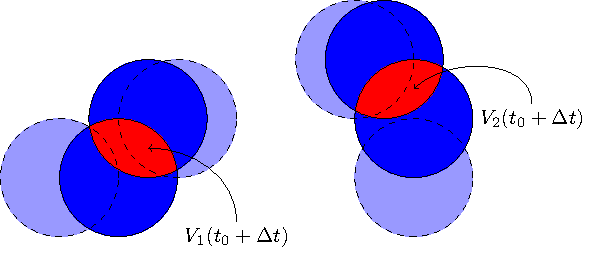
\includegraphics{figures/collisions.pdf}
\end{center}
\caption{Sketch of potential collisions.}
\end{figure}
The exact solutions of the Stokes equations prohibit contact between
force-free and torque-free particles in finite time due to lubrication
forces. When evaluating a target point close to the boundary (as is necessary when two particles come close together) the kernel in the double layer potential becomes very sharply peaked and thus difficult to integrate accurately. Spatial and temporal adaptivity \cite{Kropinski1999}, special integration techniques \cite{Klockner2013, Ying2006} or asymptotic expansions of lubrication forces \cite{Mammoli2006} are all tools that can help, however even if we evaluate the double layer potential accurately, time stepping errors can still lead to contact. To keep computational costs reasonable we must turn to alternative approaches. 

One such approach is to introduce an artificial repulsion force. There
are many possible choices for the type of force. One possibility is a repulsion force based on a Morse or 
Lennard -Jones type potential that grows as a high order polynomial as two particles become close together \cite{Flormann2017, Liu2006}. This has been shown to work for dense
suspensions, however the resulting ODEs become very stiff as the
separation between particles decreases, thus requiring smaller time
steps. Spring based models \cite{Tsubota2006, Zhao2013, Kabacogulu2017} have also been used to generate artificial repulsion forces.

Our approach mirrors \cite{Lu2017} whereby we choose the forces in such a way as to
explicitly guarantee each time step is collision free.  At each time
step $t^n$ the Stokes equations are solved and the particles are
advanced to a candidate configuration at $t^{n+1}$.  Using a linear
interpolant, we check if any collisions occurred in the interval
$[t^n,t^{n+1}]$.  If the time step is contact-free, the candidate
configuration is accepted.  If contact is detected, the candidate
solution is rejected and we resolve
equations~\eqref{eqn:vel_walls},~\eqref{eqn:vel_particles},
and~\eqref{eq:closure}, but with artificial repulsion forces $\FF^\gamma_j$ and torques
$L^\gamma_j$ that are chosen to try and avoid contact.  This lets us form a new candidate configuration. This process is repeated until we end up with a contact-free configuration.


%%%%%%%%%%%%%%%%%%%%%%%%%%%%%%%%%%%%%%%%%%%%%%%%%%%%%%%%%%%%%%%%%%%%%%%%%%%%%%%
\subsection{Avoiding Contact with STIV}
Before discussing how collisions can be resolved, we first define a
metric that measures collision.  This metric should track all pairwise
collisions and detect if a two particles overlapped not only at the
discrete time points, but at any time.  We let $\mathbf{V}(t)$ be a
vector with size $\binom{M_p}{2}$ which is the total number of possible
pairwise collisions.  $\mathbf{V}$ should be defined in such a way that
it is 0 if no collisions have occurred, and if there is a collision, its
value should quantify the amount of overlap.   Then, if there is a
collision between two particles, the repulsion force should be chosen to
scale with the magnitude of the corresponding entry of $\mathbf{V}$.
There are several possible choices for $\mathbf{V}(t)$, the simplest
being a signed distance between all points on all particles. We use the
concept of {\em Space-Time Interference Volumes} (STIV) introduced by
Harmon et al.~\cite{Harmon2011} and adapted for the suspension of
deformable and rigid particles~\cite{Lu2017}. STIVs involve a time integral and
are therefore more expensive to compute than other metrics (e.g. a signed
distance). In most simulations however the cost of computing an STIV is dwarfed by the cost of the linear solves necessary to compute the velocities of the particles. The advantage of STIVs compared to simpler metrics is that under the assumption of
ballistic motion they are able to detect collisions between two particles that
pass completely through one another, i.e. it can detect that a collision has occured even if the final candidate configuration is contact-free.





%%%%%%%%%%%%%%%%%%%%%%%%%%%%%%%%%%%%%%%%%%%%%%%%%%%%%%%%%%%%%%%%%%%%%%%%%%%%%%%
\subsection{Variational Formulation}

The incompressible Stokes equations can be can be restated as a minimization
problem. Consider the functional,
\[ \mathcal{J}(\mathbf{u}) = \int_{\Omega} \nabla\mathbf{u}:\nabla\mathbf{u} -
2\mathbf{f}\cdot\mathbf{u} ~\text{d}\Omega,\]
and the associated constrained minimization problem,
\[ \min \mathcal{J}(\mathbf{u}) ~:~ \nabla\cdot\mathbf{u} = 0 \text{ in
}\Omega.\]
Introducing $p$, a Lagrange multiplier for the incompressibility condition, we
can construct a Lagrangian for this system,
\begin{equation}\label{eq:lagrangian} \mathcal{L}(\mathbf{u},p) =
\mathcal{J}(\mathbf{u}) - \int_{\Omega}
2p\nabla\cdot\mathbf{u}~\text{d}\Omega.\end{equation}
First order optimality (KKT) conditions for $\mathcal{L}(\mathbf{u},p)$ recover
the incompressible Stokes equations. For our problem, in addition to the
incompressibility condition, we wish to enforce the constraint that the solution $\mathbf{u}$ at a time $t_0$ should not introduce collisions at time $t_0+\Delta t$, in other words $\mathbf{V}(t_0 + \Delta t) \geq \mathbf{0}$.
This constraint can be incorporated in the Lagrangian \eqref{eq:lagrangian} with the introduction of a Lagrange multiplier $\pmb{\lambda}$ with one component foreach possible collision volume,
\begin{equation}\label{eq:lagrangian2} \tilde{\mathcal{L}}(\mathbf{u},p,\lambda)= \mathcal{L}(\mathbf{u},p) + \pmb{\lambda} \cdot \mathbf{V}(t_0+\Delta
t).\end{equation}
First order optimality for \eqref{eq:lagrangian2} yields the Stokes equations
with a modified forcing function,
\begin{equation}\label{eq:stokes_mod}-\Delta \mathbf{u} + \nabla p = \mathbf{f}
+ \int_{\Omega} \text{d}_{\mathbf{u}} \mathbf{V}^T\pmb{\lambda}
~\text{d}\Omega,\end{equation}
subject to the constraints
\[ \nabla\cdot\mathbf{u} =0, ~\mathbf{V}(t_0 + \Delta t) \geq 0,~\pmb{\lambda}
\geq 0, ~ \pmb{\lambda}\cdot\mathbf{V}(t_0+\Delta t) = 0. \]

The constraints on $\mathbf{V}$ and $\pmb{\lambda}$ can be combined into a
single constraint,
\begin{equation}\label{eq:ncp_constraint} \mathbf{V}(t_0 + \Delta t)\geq
\mathbf{0} \perp \pmb{\lambda}\geq \mathbf{0}.\end{equation}


%%%%%%%%%%%%%%%%%%%%%%%%%%%%%%%%%%%%%%%%%%%%%%%%%%%%%%%%%%%%%%%%%%%%%%%%%%%%%%%
\subsection{Incorporating Repulsion Forces}

The addition of a forcing term to the right hand side of the Stokes equations
would normally lead to a volume integral. However, in this case since
$\text{d}_{\mathbf{u}} V$ can be non-zero only on the boundary, we can capture
the repulsion force by adding a net force and torque to each particle or wall as needed. The net force $\mathbf{F}^k_p$ and torque $L^k_p$ are given by,
\[ \mathbf{F}^k_p = \int_{\Gamma_k}
\text{d}_\mathbf{u}V^T\pmb{\lambda}~\text{d}s, \qquad L_p^k = \int_{\Gamma_k}
\text{d}_\mathbf{u}V^T\pmb{\lambda}\cdot(\mathbf{x}-\mathbf{c}_k)^\perp~\text{d}s.\]

%%%%%%%%%%%%%%%%%%%%%%%%%%%%%%%%%%%%%%%%%%%%%%%%%%%%%%%%%%%%%%%%%%%%%%%%%%%%%%%
\subsection{Complementary Problem}

To compute the repulsion forces we must first compute $\pmb{\lambda}$ for each
time step such that \eqref{eq:ncp_constraint} is satisfied.
Consider particles suspended in a fluid in an ambient flow $\mathbf{u}_\infty$.
This flow can be an imposed background flow or come from solid walls. In the
later case this velocity field is computed by solving the appropriate resistance problem. In either case this flow can be expressed as the sum of a translational component $\mathbf{u}_{\infty}^\tau$, a rotational component $\omega_{\infty}$ and a strain component $\mathbf{e}_{\infty}$,
\[ \mathbf{u}_{\infty}(\mathbf{x}) = \mathbf{u}_{\infty}^\tau +
\omega_\infty\times \mathbf{x} + \mathbf{e}_\infty \cdot\mathbf{x}.\]
The translational and rotational velocity as well as the density
function of a collection of particles can be computed from the force,
torque and strain rate~\cite{Karrila1991},
\begin{equation}\label{eq:mobility} \begin{bmatrix} \mathbf{u}_\infty^\tau -
\mathbf{u}_\tau\\ \omega^\infty - \omega \\\pmb{\eta}\end{bmatrix} =
\mathcal{M}\begin{bmatrix}\mathbf{F}\\\mathbf{L}\\\mathbf{e}_\infty\end{bmatrix},\end{equation}
where $\mathcal{M}$ is the {\em mobility tensor} and depends only on the
particle configuration $\mathbf{q}^0$ at some time $t^0$. Assuming the
only force and torques acting on particles arises from repulsion forces,
we can decompose \eqref{eq:mobility} as,
\[ \begin{bmatrix} \mathbf{u}_\infty^\tau - \mathbf{u}_\tau\\ \omega^\infty -
\omega \\\pmb{\eta}\end{bmatrix} =
\mathcal{M}\begin{bmatrix}\mathbf{0}\\\mathbf{0}\\\mathbf{e}_\infty\end{bmatrix}+
\mathcal{M}\begin{bmatrix}\mathbf{F}_c\\\mathbf{L}_c\\\mathbf{0}\end{bmatrix}.\]
Once we solve for $\mathbf{u}_\tau$ and $\omega$ we can update the positions an dangles of each particle using an explicit Euler step. With an abuse of notation,
this lets us express a candidate configuration $\mathbf{q}^{1}$ as,
\[ \mathbf{q}^{1} = \mathbf{q}^n + \Delta
t\left(\mathcal{M}\begin{bmatrix}\mathbf{0}\\\mathbf{0}\\\mathbf{e}_\infty\end{bmatrix}
+
\mathcal{M}\begin{bmatrix}\mathbf{F}_c\\\mathbf{L}_c\\\mathbf{0}\end{bmatrix}\right).\]

This candidate configuration must satisfy the constraint
\eqref{eq:ncp_constraint}, which we will rewrite to show the dependence of
$\mathbf{V}$ on both $\mathbf{q}^0$ and $\mathbf{q}^{1}$,
\begin{equation}\label{eq:ncp_new}\mathbf{V}(\mathbf{q}^0,\mathbf{q}^{1})\geq
\mathbf{0}\perp \pmb{\lambda}^n\geq \mathbf{0} \Rightarrow
\mathbf{V}\left(\mathbf{q}^0, \mathbf{q}^0 + \Delta
t\left(\mathcal{M}\begin{bmatrix}\mathbf{0}\\\mathbf{0}\\\mathbf{e}_\infty\end{bmatrix}
+
\mathcal{M}\begin{bmatrix}\mathbf{F}_c\\\mathbf{L}_c\\\mathbf{0}\end{bmatrix}\right)\right)
\geq \mathbf{0} \perp\pmb{\lambda}\geq \mathbf{0} .\end{equation}

This is a nonlinear complementary problem (NCP). We can see this by explicitly
including the dependence of $\mathbf{V}$ on $\pmb{\lambda}$,
\[\mathbf{V}\left(\mathbf{q}^0, \mathbf{q}^0 + \Delta
t\left(\mathcal{M}\begin{bmatrix}\mathbf{0}\\\mathbf{0}\\\mathbf{e}_\infty\end{bmatrix}
+ \mathcal{M}\begin{bmatrix} \int_{\Gamma_k}
\text{d}_\mathbf{u}\mathbf{V}^T\pmb{\lambda}~\text{d}s\\ \int_{\Gamma_k}
\text{d}_\mathbf{u}\mathbf{V}^T\pmb{\lambda}\cdot(\mathbf{x}-\mathbf{c}_k)^\perp~\text{d}s
\\\mathbf{0}\end{bmatrix}\right)\right) \geq \mathbf{0} \perp\pmb{\lambda}\geq
\mathbf{0} .\]

A first order linearization of this NCP turns it into a sequence of linear
complementary problems (LCP). Starting from an initial guess for
$\pmb{\lambda}$, $\pmb{\lambda}^0$ the following sequence should converge to the solution of \eqref{eq:ncp_new}:
\begin{equation}\label{eq:lcp}\begin{aligned}
\mathbf{V}\biggl(\mathbf{q}^0 + \Delta
t\biggl(\mathcal{M}\begin{bmatrix}\mathbf{0}\\\mathbf{0}\\\mathbf{e}_\infty\end{bmatrix}
&+ \mathcal{M}\begin{bmatrix} \int_{\Gamma_k}
\text{d}_\mathbf{u}\mathbf{V}^T\pmb{\lambda}^\ell~\text{d}s\\ \int_{\Gamma_k}
\text{d}_\mathbf{u}\mathbf{V}^T\pmb{\lambda}^\ell\cdot(\mathbf{x}-\mathbf{c}_k)^\perp~\text{d}s
\\\mathbf{0}\end{bmatrix}\biggr)\biggr) \\
&+ \Delta t \mathcal{M}\begin{bmatrix}\int_{\Gamma_k}
\text{d}_\mathbf{u}\mathbf{V}^T\pmb{\lambda}^{\ell+1}~\text{d}s\\
\int_{\Gamma_k}
\text{d}_\mathbf{u}\mathbf{V}^T\pmb{\lambda}^{\ell+1}\cdot(\mathbf{x}-\mathbf{c}_k)^\perp~\text{d}s
\\\mathbf{0}\end{bmatrix}\frac{\partial\mathbf{V}}{\partial \mathbf{q}^1} \geq
\mathbf{0} \perp \pmb{\lambda}^{\ell+1} \geq
\mathbf{0}.\end{aligned}\end{equation}

The sequence \eqref{eq:lcp} will be solved at each time step. 

\subsection{Computing Pressures and Stresses}

Once we have computed the density function $\pmb{\eta}$ we can use it to post-process various other quantities of interest, for example pressure, stress or energy dissipation. 

From the velocity we can compute the pressure, by solving the equation
\begin{equation*}\nabla p = \Delta \mathbf{u} .\end{equation*}
Looking at the 1st component of this equation we get
\begin{equation*}\frac{\partial p}{\partial x} = \Delta u \Rightarrow p(x,y) = \int \Delta u \text{d}x + f(y).\end{equation*}
We can take $f(y)$ to be 0 since there is no reason for pressure to have a preferred direction. Using \eqref{eq:completed_DLP} we can compute this quantity,
\begin{equation}\label{eq:pressure} p(\xx) = \frac{1}{\pi}\int_{\partial\Omega}\frac{1}{\rho^2}\left(( \mathbf{I} - 2(\rr \otimes \rr)\nn\right)\cdot\pmb{\eta}~\text{d}s + \sum\limits_{i=1}^{M_w} \frac{\mathbf{F}_i^\Gamma\cdot(\mathbf{x}-\mathbf{c}_i)}{2\pi||\mathbf{x}-c_i||^2}  + \sum\limits_{j=1}^{M_p} \frac{\mathbf{F}_j^\gamma\cdot(\mathbf{x}-\mathbf{c}_j)}{2\pi||\mathbf{x}-c_j||^2}.\end{equation}


The stress tensor for a Newtonian fluid with unit viscosity is given by
\begin{equation*} \pmb{\sigma} = -p \mathbf{I} + \left(\nabla \uu + (\nabla\uu)^T\right).\end{equation*}
Using the pressure computed in \eqref{eq:pressure} and computing the viscous part of the stress tensor from \eqref{eq:completed_DLP} we get
\begin{equation}\label{eq:stress} \ssigma = \ssigma_{\eeta} + \ssigma_{S} + \ssigma_{R},\end{equation}
where
\begin{align*}\ssigma_{\eeta}(\xx) &= \frac{1}{\pi}\int_{\partial\Omega}\left( \frac{\nn\cdot\eeta}{\rho^2}\mathbf{I} -\frac{(\rr\cdot\nn)(\rr\cdot\eeta)(\rr\otimes\rr)}{\rho^6} + \frac{(\rr\cdot\nn)(\rr\otimes\eeta + \eeta\otimes\rr)}{\rho^4} + \frac{(\rr\cdot\eeta)(\rr\otimes\nn + \nn\otimes\rr)}{\rho^4}\right)\text{d}s,\\
\ssigma_S(\xx) &= \sum\limits_{i=1}^{M_w} \frac{\mathbf{F}_i^\Gamma\cdot(\mathbf{c}_i-\mathbf{x})}{\pi||\mathbf{x}-c_i||^2}(\cc_i - \xx)\otimes(\cc_i-\xx)  + \sum\limits_{j=1}^{M_p} \frac{\mathbf{F}_j^\Gamma\cdot(\mathbf{c}_j-\mathbf{x})}{\pi||\mathbf{x}-c_j||^2}(\cc_j - \xx)\otimes(\cc_j-\xx),\\
\ssigma_R(\xx) &= \sum\limits_{i=1}^{M_w} \frac{L_i^\Gamma}{2\pi||\mathbf{x}-c_i||^2}((\cc_i - \xx)\otimes(\cc_i-\xx)^\perp + (\cc_i - \xx)^\perp\otimes(\cc_i-\xx))  \\&\qquad\qquad\qquad + \sum\limits_{j=1}^{M_p}  \frac{L_j^\gamma}{2\pi||\mathbf{x}-c_j||^2}((\cc_j - \xx)\otimes(\cc_j-\xx)^\perp + (\cc_j - \xx)^\perp\otimes(\cc_j-\xx)) .
\end{align*}

		
%%%%%%%%%%%%%%%%%%%%%%%%%%%%%%%%%%%%%%%%%%%%%%%%%%%%%%%%%%%%%%%%%%%%%%%
\section{Numerical Methods\label{s:method}} 
We use a Lagrangian formulation where we track the centers $\cc_i$ and
orientations $\theta_i$ of each rigid body $\gamma_i$.  We use a fully
implicit time stepping method and a spectral discretization in space.  All
the integral equations are discretized with a Nystr\"om  methods, and
interactions between nearly touching interfaces is resolved with a
near-singular integration scheme.  Finally, the Fast Multipole Method
(FMM) is used to accelerate the matrix-vector multiplications that arise
upon discretization.  By using these methods, spectral accuracy can be
achieved for long time horizons with optimal complexity.

%%%%%%%%%%%%%%%%%%%%%%%%%%%%%%%%%%%%%%%%%%%%%%%%%%%%%%%%%%%%%%%%%%%%%%%
\subsection{Spatial Discretization}
Letting $\xx(\alpha)$ be a parameterization of a rigid body or a solid
wall, we can represent any smooth function defined on this curve using a
Fourier series as
\begin{align}
  f(\alpha) = f(\xx(\alpha)) = \sum_{k \in \ZZ} \hat{f}_k e^{ik\alpha}.
\end{align}
The FFT is used to compute $\hat{f}$, and all derivatives are computed
with this Fourier series so that spectral accuracy is achieved.

The double-layer potentials in~\eqref{eq:vel_walls}
and~\eqref{eq:vel_particles} are discretized with a Nystr\"om method.
Because the kernels are smooth, the trapezoid rule guarantees spectral
accuracy~\cite{tre-wei2014}.  For example,
equation~\eqref{eqn:vel_walls} is discretized as
\begin{equation*}
  \begin{aligned}
  \uu_b(\xx_j) = -\frac{1}{2}\eeta(\xx_j) + 
  \sum_{k=1}^{N} K(\xx_j,\xx_k) \eeta(\xx_k) \Delta s_k
    &+ \sum_{i=1}^{M} \left(\mathbf{S}(\xx_j,\dd_i)\llambda_i +
    \mathbf{R}(\xx_j,\dd_i)\mu_i\right)  \\
    &+ \sum_{i=1}^{N} \left(\mathbf{S}(\xx_j,\cc_i)\FF_i +
    \mathbf{R}(\xx_j,\cc_i)\L_i\right),
  \end{aligned}
\end{equation*}
where $N = M_w N_w + M_p N_p$ is the total number of discretization
points and
\begin{align*}
  K(\xx,\yy) = \frac{1}{\pi} \frac{\rr \cdot \nn}{\rho^2} 
               \frac{\rr \otimes \rr}{\rho^2}
\end{align*}
is the kernel of the double-layer potential.
Equation~\eqref{eq:vel_particles} is discretized in a similar fashion.
For the diagonal entries, we use the limiting value of $K$
\begin{align*}
  \lim_{\substack{\yy \rightarrow \xx \\ \yy \in \bd\Omega}} K(\xx,\yy) = 
    \text{whatever it is involving the curvature and tangent vector},
    \quad \xx \in \bd\Omega
\end{align*}
where $\kappa(\xx)$ is the curvature and $\tt(\xx)$ is the tangent
vector of $\bd\Omega$ at $\xx$.

The trapezoid rule achieves spectral accuracy when both the source
points $\yy$ and the target point $xx$ are on the same solid wall
$\Gamma_k$ or rigid particle $\gamma_k$.  However, when the target point
is on a different body, the accuracy of the trapezoid rule can
deteriorate which leads to instabilities.  This increase in error
happens when the target point is close to the source points, but not on
the same body as the source points.  To resolve this issue, an algorithm
for near-singular integration method must be employed.  There are now
several methods for near-singular integration including
regularizations~\cite{bea-yin-wil2016, bea-lai2001}, quadrature by
expansion~\cite{Klockner2013}, barycentric
interpolation~\cite{bar-wu-vee2015}, and panel-based
quadrature~\cite{hel-oja2008}.  In this work, we use an interpolation
based scheme~\cite{Ying2006} which has been used for other
two-dimensional suspensions~\cite{Quaife2014}.

Once each of the
equations~\eqref{eq:vel_walls},~\eqref{eq:vel_particles},
and~\eqref{eq:closure} have been discretized using the above described
quadrature rules, the result is a dense $N \times N$ linear system.
Since this linear system is the discretization of a second-kind integral
equation, GMRES~\cite{Saad1986} converges in a mesh-independent number of
iterations~\cite{cam-ips-kel-mey-xue1996}.  Since GMRES only requires
matrix-vector multiplications, the algorithmic cost per time step is
proportional to the cost of doing a single matrix-vector multiply.




%%%%%%%%%%%%%%%%%%%%%%%%%%%%%%%%%%%%%%%%%%%%%%%%%%%%%%%%%%%%%%%%%%%%%%%
\subsection{Time Discretization}



%%%%%%%%%%%%%%%%%%%%%%%%%%%%%%%%%%%%%%%%%%%%%%%%%%%%%%%%%%%%%%%%%%%%%%%
\subsection{Fast Summation Methods}




The linear system \eqref{eq:stokes_unbounded} or
\eqref{eq:stokes_bounded} is discretized using a collocation trapezoid
method. For particles that are in near-contact the near singular
integration scheme described in~\cite{Quaife2014, Ying2006} is used. The
discretized system is solved with GRMES~\cite{Saad1986} with a block
diagonal preconditioner and accelerated using the fast multipole method
\cite{Greengard1987}.  Since the linear system arises from a second kind
Fredholm equation the condition number of the matrix is bounded and does
not increase with finer resolution. The number of GMRES iterations is
therefore mesh resolution independent. This leads to a solver that is
$O(n)$, where $n$ is the number of mesh points. 

Once we solve for the translational and angular velocity of the
particles, the position and angle of each particle are updated according
to the ODEs,
\[ \frac{\text{d}}{\text{d}t}\mathbf{c}_k = \mathbf{u}^\tau_k, \qquad
\frac{\text{d}}{\text{d}t}\theta_k =\omega_k.\]
The ODEs are advanced in time using an explicit Euler step. 

The matrices described in \eqref{eq:stokes_unbounded} and
\eqref{eq:stokes_bounded} are full. They can be made block-diagonal by
treating inter-particle interactions explicitly and moving them to the
right hand side. This is termed {\em locally implicit} and is described
in \cite{Lu2017}. For dense suspensions however this type of time
stepping can lead to instabilities as particles become tightly packed. 

\begin{algorithm}
	 \SetKwInOut{Input}{Input}
    	\SetKwInOut{Output}{Output}

  	  \underline{Collision free time stepper}\;
\Input{collision free configuration $\mathbf{q}^0$, time step size $\Delta t$}
\Output{collision free configuration $\mathbf{q}^1$ }
	 $\mathbf{u}^* \gets \mathbf{A}(\mathbf{q}^0,\mathbf{0},\mathbf{0})$\;
	$\mathbf{q}^* \gets \mathbf{q}^0 + \Delta t \mathbf{u}^*$\;
	Compute $\mathbf{V}(\mathbf{q}^0,\mathbf{q}^*)$, $\text{d}_u\mathbf{V}$\;
	\While {$\mathbf{V} < \mathbf{0}$}
	{
		$\pmb{\lambda} \gets$ LCP\_solve($\text{d}_{\mathbf{u}}\mathbf{V}$)\;
$\mathbf{F}_k \gets \int_{\Gamma_k}
\text{d}_{\mathbf{u}}\mathbf{V}^T\pmb{\lambda}~\text{d}s$\;
$L_k \gets \int_{\Gamma_k}
\text{d}_{\mathbf{u}}\mathbf{V}^T\pmb{\lambda}\cdot(\mathbf{x}-\mathbf{c}_k)^\perp~\text{d}s$\;
		$\mathbf{u}^* \gets \mathbf{A}(\mathbf{q}^0,\mathbf{F}_k,\mathbf{L}_k)$\;
		$\mathbf{q}^* \gets \mathbf{q}^0 + \Delta t \mathbf{u}^*$\;
		Compute $\mathbf{V}(\mathbf{q}^0,\mathbf{q}^*)$, $\text{d}_u\mathbf{V}$\;
	}
\end{algorithm}

%%%%%%%%%%%%%%%%%%%%%%%%%%%%%%%%%%%%%%%%%%%%%%%%%%%%%%%%%%%%%%%%%%%%%%%
\section{Results\label{s:results}} 

\subsection{Shear Flow}

A simple numerical experiment done in \cite{Lu2017} is repeated with our globally implicit time stepper. Two particles are placed in an unbounded shear flow, $\mathbf{u}^\infty = (y, 0)$. The rightmost particle is placed on the origin, while the leftmost particle is placed slightly above the $y$ axis at $(-8, 0.5)$. As the particles come close to each other the left particle is deflected above the right one and continues on a trajectory to the right with a constant $y$ value. The particles are discretized with 32 points, meaning that the arc length spacing is $2\pi/32 \approx 0.196$. In this experiment the particles never get within $2h$ of one another, meaning that if we take $\delta$ to be less than $2h$ the collision constraint is not necessary. 
\begin{figure}[!h]
\begin{center}
\includegraphics{figures/shear_setup1.pdf}
\begin{tabular}{c c}
\includegraphics{figures/shear_displacement1.pdf} &
\includegraphics{figures/separation_displacement1.pdf}
\end{tabular}
\end{center}
\caption{Shear experiment. Top: initial setup and trajectories of the centers of both rigid bodies. Bottom left: the $y$ coordinate of the center of the particle initially on the left as a function of its horizontal displacement. Bottom right: the final vertical displacement of the particle initially on the right as a function of separation distance.}\label{fig:shear_experiment}
\end{figure}

We can use this setup to look at effect of the contact force on the time reversibility of the flow. By reversing the shear direction at $t=10$ we can measure the relative error between the initial particle center and the particle center at $t=20$. The results for various value of $\delta$ are shown in table \ref{tab:reverse}. For $\delta = 0$ (no contact constraint) we get first order accuracy in the reversibility of the flow. This is expected as we are using forward Euler as our time stepper. For $\delta \geq 2$ we see that we no longer recover reversibility. This is due to the fact that the force has the no the effect of shifting the particles onto a streamline that is contact free. If we reverse the direction of the flow we will be traversing this contact-free streamline. 

\begin{table}[!h]
\begin{center}
\begin{tabular}{c| c c c c c}
$ $ & & & $\Delta t$ & &\\
$h$ & $4\e{-2}$ &$ 2\e{-2}$ & $1\e{-2}$ & $5\e{-3}$ & $2.5\e{-3}$\\
\hline
0 & $1.35\e{-1}$ & $7.32\e{-2}$ & $3.74\e{-2}$ & $2.00\e{-2}$ & $1.01\e{-2}$\\
$2h$ & $1.88\e{-1}$ & $1.41\e{-1}$ & $1.17\e{-1}$ & $1.08\e{-1}$ & $1.02\e{-1}$\\
$2.25h$ & $2.55\e{-1}$ & $2.08\e{-1}$ & $1.87\e{-1}$ & $1.78\e{-1}$ & $1.73\e{-1}$\\
$2.50h$ & $3.05\e{-1}$ & $2.69\e{-1}$ & $2.52\e{-1}$ & $2.45\e{-1}$ & $2.40\e{-1}$\\
$2.75h$ & $3.64\e{-1}$ & $3.31\e{-1}$ & $3.13\e{-1}$ & $3.07\e{-1}$ & $3.03\e{-1}$\\
$3.00h$ & $4.12\e{-1}$ & $3.88\e{-1}$ & $3.72\e{-1}$ & $3.67\e{-1}$ & $3.63\e{-1}$
\end{tabular}
\end{center}
\caption{Study of time reversibility of the shear flow setup depicted in figure \ref{fig:shear_experiment}. At $t=10$ the flow direction is reversed and we calculate the relative error in the starting position and the position at $t=20$. When the collision constraint is active and force is needed to keep the particles apart we no longer recover time reversibility.}\label{tab:reverse}
\end{table}


\subsection{Taylor-Green}

One of the advantages of using a globally implicit time stepper is that it can handle dense suspensions without requiring an excessively small time step. We will look at a dense suspension of 75 rigid particles in unbounded Taylor-Green flow. The background velocity field $\mathbf{u}^\infty$ is given by $(\cos(x)\sin(y), -\sin(x)\cos(y))$. Snapshots of the simulation are shown in figure \ref{fig:taylor_green}. 

\begin{figure}[!h]
\begin{center}
\begin{tabular}{c c c c}
\includegraphics[width=3cm]{figures/taylor_green0.pdf} &
\includegraphics[width=3cm]{figures/taylor_green1.pdf}&
\includegraphics[width=3cm]{figures/taylor_green2.pdf} &
 \includegraphics[width=3cm]{figures/taylor_green_tracks.pdf}
\end{tabular}
\end{center}
\caption{Dense suspension in unbounded Taylor-Green flow. Particles are discretized with 32 points and a minimum separation of $0.05h$ is enforced. Snapshots of the simulation at $t=0$, $t=15$ and $t=30$ are shown. The bottom right plot shows the track of the center of the particle shaded in magenta for different time step sizes. Each line in that plot is marked where a repulsion force is necessary to enforce the minimum separation. }\label{fig:taylor_green}
\end{figure}

\subsection{Taylor-Couette}

We can use our model to investigate rheological properties of suspensions. Here we will look at suspensions of varying volume fraction and particle aspect ratio; specifically we will look at 5 and 10 percent volume fractions and ellipse shaped particles of aspect ratio 3 to 1 and 6 to 1. Initially the particles are placed randomly inside the device; the initial configurations are shown in figure \ref{fig:couette_setup}. 

\begin{figure}[!h]
\begin{center}
\begin{tabular}{c c c c}
\includegraphics[width=3cm]{figures/couette_005_3_1.pdf} & \includegraphics[width=3cm]{figures/couette_005_6_1.pdf} &
\includegraphics[width=3cm]{figures/couette_010_3_1.pdf} & \includegraphics[width=3cm]{figures/couette_010_6_1.pdf}
\end{tabular}
\end{center}
\caption{Four initial configurations for Taylor-Couette flow with varying volume fraction $\phi$ and aspect ratio $r$. From left to right: 1) $\phi=5\%$, $r = 3:1$, 2) $\phi=5\%$, $r=6:1$, 3) $\phi=10\%$, $r=3:1$, 4) $\phi=10\%$, $r=6:1$.}\label{fig:couette_setup}
\end{figure}

By measuring the torque on the inner cylinder we can get an instantaneous value of the effective viscosity of the suspension. As can be seen in figure \ref{fig:torque}, the effective viscosity increases with $\phi$, but is generally lower with the 6 to 1 shaped particles.
\begin{figure}[!h]
\begin{center}
\includegraphics{figures/couette_torque.pdf}\\
\end{center}
\caption{Instantaneous effective viscosity for the cases shown in figure \ref{fig:couette_setup}. The inner cylinder is fixed, while the outer one spins. The ratio of the torque on the inner cylinder to the baseline torque (i.e. the torque on the inner cylinder of a device with no particles) gives the instantaneous effective viscosity.}\label{fig:torque}
\end{figure} 

Another quantity we may be interested is the alignment of the particles. On average we expect the particles to align in the direction of the shear flow, which in this case is the $\hat{\theta}$ direction. Figure \ref{fig:angles} shows the deviation from this expected orientation as a function of time for the four cases. We see that the 5\% volume fractions align quicker than the 10\% volume fractions. 

\begin{figure}[!h]
\begin{center}
\includegraphics{figures/couette_angle_mean.pdf}\\
\end{center}
\caption{Deviation from the expected alignment angle. }\label{fig:angles}
\end{figure} 

\begin{figure}[!h]
\begin{center}
\includegraphics{figures/pressure_contour.pdf}
\end{center}
\caption{Pressure distribution inside a Couette device. The outer cylinder is spinning while the inner cylinder is fixed. }\label{fig:dissipation}
\end{figure}
%%%%%%%%%%%%%%%%%%%%%%%%%%%%%%%%%%%%%%%%%%%%%%%%%%%%%%%%%%%%%%%%%%%%%%%
\section{Conclusions\label{s:conclusions}}


%%%%%%%%%%%%%%%%%%%%%%%%%%%%%%%%%%%%%%%%%%%%%%%%%%%%%%%%%%%%%%%%%%%%%%%
\begin{appendices}
An appendix
\end{appendices}


\bibliographystyle{plainnat} 
\bibliography{bibliography}
\biboptions{sort&compress}
\end{document}
